\chapter{神经符号框架的架构设计与实现}
\section{引言}
本章对神经符号框架的架构进行详细的介绍,包括流水线总体架构、视觉场景理解、语义解析、迭代反馈和规则修正、规则蒸馏、ASP推理等模块的设计和实现。
框架的设计目标如下:
\begin{enumerate}[label=(\arabic*),itemsep=0pt,parsep=0pt]
\item 借鉴已有的神经符号框架的设计思路,添加、修改部分模块,提升框架对ASP规则的自动拓展能力,进而进一步增强VQA系统回答部分可见问题的准确率。
\item 使用Dspy来完成对LLM的提示、优化,以降低神经符号方法的开发难度。
\end{enumerate}
\section{框架总体架构}
框架的总体架构如图\ref{fig:pipeline}所示。其中,LLM在整个框架中的作用有以下两点:
\begin{enumerate}[label=(\arabic*),itemsep=0pt,parsep=0pt]
    \item 在语义解析模块中,LLM对自然语言问题进行语义解析,将问题以ASP的形式表示出来,以便后续
输入到迭代反馈模块中进行修正。
    \item 在迭代反馈模块中,LLM对ASP表示进行多次迭代优化,其中包括解析错误、基础化错误等。每一轮迭代都将
根据上一轮的错误信息进行针对性的修正。
    \item 在规则蒸馏中,LLM结合ASP知识库中的先验知识,对迭代反馈修正后ASP规则进行进一步补全,为Clingo求解器
推理提供更全面的知识。
    \item 在求解结果翻译中,LLM对Clingo求解器输出的以ASP表示的结果进行翻译,使其以自然语言形式,针对提出的问题
进行作答。
\end{enumerate}
\begin{figure}
    \centering
    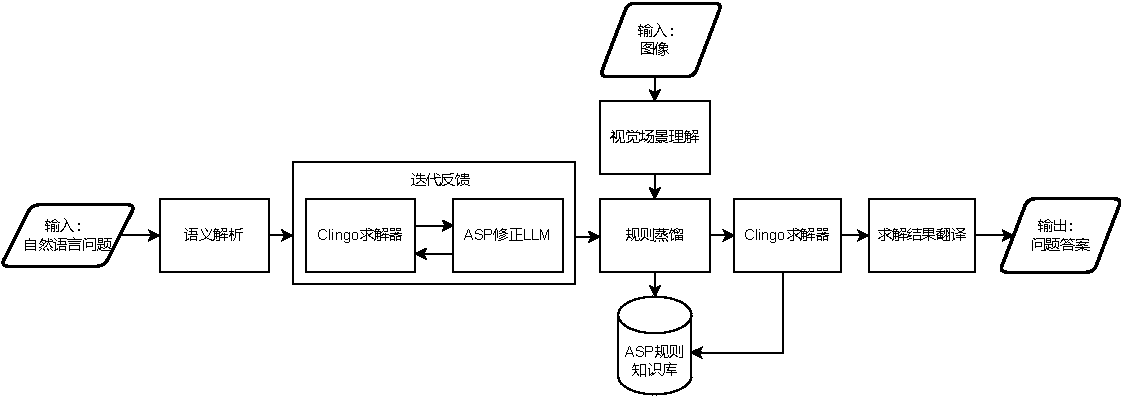
\includegraphics[width=\textwidth]{figures/pipeline-crop.pdf}
    \caption{面向空间推理领域的神经符号框架示意图}
    \label{fig:pipeline}
\end{figure}
本文在语义解析模块和迭代反馈模块中,分别采用不同的LLM,各自进行微调,以更好地满足不同任务的需求。
\section{视觉场景理解}
视觉场景理解是本文所设计流水线中的核心模块,其目标是从输入图像中提取结构化信息,包括物体的属性(如形状、颜色、大小等)、位置信息以及物体间的空间关系。这些信息将被进一步转换为ASP的形式,为后续基于逻辑推理的语义解析与问答模块提供形式化的知识基础。

本章主要围绕以下四个方面展开详细阐述:目标检测、空间位置提取、空间关系提取以及场景图生成。最后,本文给出一个完整的视觉场景理解演示案例,并讨论在实现过程中遇到的关键技术挑战及相应解决方案。
\subsection{目标检测}
目标检测是视觉场景理解的最基础的任务,其目标是从图像中识别出所有相关物体,并标注其边界框、类别和属性。本文选择GLIP模型作为目标检测的实现工具,原因在于
其独特的语言-视觉预训练特性。基于大规模的图文对数据,GLIP进行大量预训练,能够根据自然语言描述(如“红色立方体”)直接定位图像中的对应物体。
这种能力特别适合VQA任务,使问题中的语言信息与图像内容高效对齐成为可能。

目标检测是视觉场景理解的基础任务,其任务是从输入图像中识别出所有相关物体,
并为每个物体确定其边界框、类别和相关属性。本文采用了GLIP模型作为目标检测的核心工具,其主要优势体现在:
\begin{enumerate}[label=(\arabic*),itemsep=0pt,parsep=0pt] 
\item \textbf{语言-视觉预训练能力:}GLIP在大规模图文对数据上进行预训练,能够根据自然语言描述(例如“红色立方体”)直接定位图像中的对应物体,从而实现图像内容与问题描述的高效对齐; 
\item \textbf{高效性与鲁棒性:}模型在处理多样化场景时具有较高的检测准确率,适合构造后续依赖视觉信息的场景图。 
\end{enumerate}

具体实现流程如下:
\begin{enumerate}[label=(\arabic*),itemsep=0pt] 
\item \textbf{图像预处理:}将原始图像调整至GLIP模型要求的输入分辨率(例如800$\times$1333像素),
以保证检测精度; 
\item \textbf{文本提示构造:}根据数据集构造要求,设计一组覆盖目标类别及属性的自然语言提示。
本文选取的提示短语包括描述物体大小(如“大物体”、“小物体”)以及颜色与形状组合(如“红色立方体”、“蓝色球体”、“绿色圆柱体”等); 
\item \textbf{目标检测与属性解析:}将图像和文本提示输入GLIP,获得每个检测物体的边界框和类别标签。随后对类别标签进行解析,将复合描述(如“红色立方体”)拆解为单独属性(color=red, shape=cube)。同时,通过计算边界框面积($(x_2 - x_1)\times(y_2 - y_1)$),结合预设阈值进一步推断物体的大小属性。 
\end{enumerate}

例如,对于一张包含“红色立方体”和“蓝色球体”的图像,GLIP可能检测出如下信息: 
\begin{enumerate}[itemsep=0pt,parsep=0pt] 
\item 物体1:类别为“红色立方体”,边界框坐标为$(x_1, y_1, x_2, y_2)$; 
\item 物体2:类别为“蓝色球体”,边界框坐标为$(x_3, y_3, x_4, y_4)$。 
\end{enumerate}
\subsection{空间位置提取}
在完成目标检测后,接下来的任务是为每个物体确定其精确的空间位置,这对于后续空间关系的推理至关重要。
本文采用以下两种方式提取物体位置信息:
\begin{enumerate}
\item \textbf{二维中心点计算}:利用目标检测得到的边界框信息,计算物体在图像平面内的中心点坐标。公式如下:
$$x_c = \frac{x_1+x_2}{2}, y_c = \frac{y_1 + y_2}{2}$$
该中心点坐标用于描述物体在二维图像中的位置;
\item \textbf{三维位置信息获取}:若图像同时包含深度信息(例如通过Blender渲染生成的场景),则可直接从深度图中提取物体的z值,从而获得物体在三维空间中的位置,
表示为$(x, y, z)$。
\end{enumerate}

提取出的位置信息将以ASP事实的形式进行存储,例如:position(obj1, x1c, y1c, z1) 表示物体1的中心点位置。
\subsection{空间关系提取}
空间关系的提取是实现复杂场景理解与多步逻辑推理的关键。本文从以下几个角度对空间关系进行提取:
\begin{enumerate}[label=(\arabic*),itemsep=0.5em] 
\item \textbf{二维空间关系:}基于物体的中心点坐标计算物体之间的相对位置。例如: 
    \begin{itemize}[leftmargin=2em] 
        \item 若物体A的$x_c$小于物体B的$x_c$,则判定A位于B的左侧,表示为\texttt{left(objA, objB)}; 
        \item 类似地,通过比较$y_c$坐标可判定上下关系(例如,若物体A的$y_c$小于B,则A在B之上,记作\texttt{above(objA, objB)})。 
    \end{itemize} 
\item \textbf{三维空间关系:}利用深度信息,对物体间的前后关系进行判断。
例如,若物体A的z值小于物体B的z值,则判定A位于B的前面,记作\texttt{in\_front\_of(objA, objB)}。 
\item \textbf{遮挡关系:}结合边界框重叠情况与深度信息进行判断。如果两个物体边界框存在重叠且A的深度值明显小于B,
则可以认为A遮挡B,记作\texttt{occludes(objA, objB)}。 
\end{enumerate}
所有提取到的空间关系均转换为ASP事实,如:
left(obj1, obj2) 表示物体1在物体2的左边,in\_front\_of(obj1, obj2) 表示物体1在物体2的前面;
occludes(obj1, obj2) 表示物体1遮挡了物体2。
\subsection{场景图生成}
场景图是将目标检测、空间位置与空间关系综合融合成的统一结构化表示,其主要构成如下: 
\begin{enumerate}[label=(\arabic*),itemsep=0.5em] 
    \item \textbf{节点表示:}每个节点对应图像中的一个物体,并附有相应的属性(如color, shape, size, material)以及位置信息; 
    \item \textbf{边的构建:}节点之间的边用于表示物体间的空间关系,如left\_of、in\_front\_of等。 
\end{enumerate}

在构建过程中,首先为每个检测到的物体创建一个节点,并记录其属性及位置;
随后,依据前述空间关系,将相应的有向边添加到图中。
最终,整个场景图将被转化为ASP事实,以支持后续符号推理任务。
\subsection{实现细节与实例}
为便于说明,下面给出一个具体示例。假设输入图像包含如下场景: 
\begin{enumerate}[label=(\arabic*),itemsep=0.5em] 
    \item 一个红色大立方体位于图像左侧; 
    \item 一个蓝色小球体位于图像右侧,且位于红色立方体的前方。 
\end{enumerate}

经过GLIP目标检测,得到如下检测结果: 
\begin{itemize}[leftmargin=2em] 
    \item 物体1:类别为“红色立方体”,边界框为(50, 100, 150, 200); 
    \item 物体2:类别为“蓝色球体”,边界框为(250, 50, 350, 150)。 
\end{itemize}

进一步计算得到: 
\begin{itemize}[leftmargin=2em] 
    \item 物体1的中心点坐标为$(100,150)$; 
    \item 物体2的中心点坐标为$(300,100)$。 
\end{itemize}

假设深度信息显示:物体1的z值为50,物体2的z值为75,则可提取以下空间关系: 
\begin{itemize}[leftmargin=2em] 
    \item \texttt{left\_of(obj1, obj2)}(因为100 $<$ 300); 
    \item \texttt{above(obj2, obj1)}(因为100 $<$ 150); 
    \item \texttt{in\_front\_of(obj2, obj1)}(因为75 $>$ 50,在三维空间中深度值较大的物体更靠后,需根据具体定义调整)。 
\end{itemize}

最终生成的ASP事实示例如下: 
\begin{lstlisting}[language=Prolog] 
color(obj1, red). 
shape(obj1, cube). 
size(obj1, large). 
position(obj1, 100, 150, 50).

color(obj2, blue). 
shape(obj2, sphere). 
size(obj2, small). 
position(obj2, 300, 100, 75).

left_of(obj1, obj2). 
above(obj2, obj1). 
in_front_of(obj2, obj1). 
\end{lstlisting}
\subsection{技术挑战与解决方案}
在实际实现过程中,本模块面临如下关键技术挑战,并提出相应解决方案: 
\begin{enumerate}[label=(\arabic*),itemsep=0.5em] 
    \item \textbf{检测准确性:}GLIP在处理物体密集或遮挡严重的场景时可能存在误检问题。为此,本文引入非极大值抑制(NMS)以及深度信息辅助过滤,提高检测精度; 
    \item \textbf{空间关系鲁棒性:}二维关系受视角影响较大,为增强鲁棒性,本文在有深度信息的条件下优先采用三维关系,并结合几何约束(例如边界框重叠)进行补充; 
    \item \textbf{计算效率:}面对大规模图像数据,为保证系统实时性,本文通过批量处理图像以及优化提示设计,有效降低了GLIP的推理延时。
\end{enumerate}
\subsection{小结}
本节详细介绍了基于GLIP的视觉场景理解模块的整体架构与实现细节。
通过对目标检测、空间位置与空间关系的综合提取,最终构建了能够转化为ASP事实的场景图,
为后续语义解析和逻辑推理提供了坚实的数据基础。
下一节将介绍如何利用LLM将自然语言问题转化为ASP查询,实现语义解析与神经符号推理的无缝衔接。
\section{语义解析}
语义解析的主要任务是,通过LLM,使用上下文学习的方法,将自然语言问题转为用ASP进行表示,获得ASP规则,以便与视觉场景理解提取的场景事实结合进行逻辑推理。

直观上,LLM可能很难直接解决复杂的推理问题。然而,LLM已经在理解文本输入并将其转化为形式化程序方面取得了巨大成功,
例如程序代码\cite{gao2023pal}和数学方程\cite{he2023solving}。为了让LLM更准确地生成ASP编码,本文在此对通用LLM进行针对性微调。
\subsection{微调数据集模板设计}
现有的通用代码生成数据集可能无法充分覆盖ASP中普遍存在的特定结构和模式,而对LLM针对特定任务进行微调,面向特定领域的数据集必不可少。
因此,对LLM针对ASP编码任务进行微调的核心是:创建一个涵盖多种ASP问题类别的微调数据集。
通过创建一个有针对性的数据集,模型可以更有效地学习这些特定的细微差别。

本文以下对常见的ASP编程任务进行分析,确定了以下9种ASP编码的基本情形,分别为其设计模板,用于后续构建微调数据集。
\subsubsection{猜测赋值}
猜测赋值是ASP编码中的经典情形。具体而言,猜测赋值指的是将某一给定集合中的所有元素赋予一个从固定集合中选出的唯一标签。
在ASP中,通常使用析取来表示“猜测”。以下是猜测赋值的一个示例。
\begin{lstlisting}
模板:为以下问题编写一个 ASP 程序。在给定的一组标签中,为元素集准确分配一个标签。元素集由谓词 [PREDICATE] 表示。标签为 [LABEL]+。
提示:为以下问题编写一个 ASP 程序。在给定的一组标签中,为元素集准确分配一个标签。元素集由谓词 city 表示。标签为 moscow、rome、dubai。
编码:assign(X,"moscow") |assign(X,"rome") | assign(X,"dubai") :- city(X).
\end{lstlisting}
\subsubsection{表达约束}
表达约束表示必须满足的条件。在ASP中,这通常通过(经典/强)约束来实现,有时会使用辅助规则。以下是表达约束的一个示例。
\begin{lstlisting}
模板:为以下问题编写一个 ASP 程序。防止值为 [VALUE] 的谓词 [PREDICATE] 带有标签 [LABEL]。
提示:为以下问题编写一个 ASP 程序。防止值为 11 的谓词 car 带有标签“red”。
编码: :- assign(11,"red").
\end{lstlisting}
\subsubsection{生成组合}
生成组合指创建来自两个不同集合的所有可能的元素组合(笛卡尔积)。在ASP中,可以通过简单的规则完成。以下是生成组合的一个示例。
\begin{lstlisting}
模板:为以下问题编写一个 ASP 程序。从两个集合生成所有元素组合。这两个集合分别由谓词 [PREDICATE_1] 和 [PREDICATE_2] 表示。
提示:为以下问题编写一个 ASP 程序。从两个集合生成所有元素组合。这两个集合分别由谓词 city 和 airport 表示。
编码: combination(X,Y) :- city(X), airport(Y).
\end{lstlisting}
\subsubsection{连接}
连接指的是基于特定匹配标准将来自两个不同集合的元素关联起来。在ASP中,通常通过在规则体中具有共享变量的文字来定义。以下是连接的一个示例。
\begin{lstlisting}
模板:为以下问题编写一个 ASP 程序。假设谓词 [PREDICATE_1] 具有字段 [LABEL]+,谓词 [PREDICATE_2] 具有字段 [LABEL]+。定义一个谓词 [PREDICATE_1]_[PREDICATE_2],将每个 [PREDICATE_1] 与 [PREDICATE_2] 的 [LABEL] 关联。
提示:为以下问题编写一个 ASP 程序。假设谓词“owner”具有字段“ID”、“surname”、“name”、“restaurantID”,谓词“restaurant”具有字段“ID”、“description”。定义一个谓词“owner_restaurant”,将每个所有者与餐厅的描述关联。
编码:owner_restaurant(X,Z) :-owner(X,_,_,Y),restaurant(Y,Z).
\end{lstlisting}
\subsubsection{传递闭包}
传递闭包用于定义超出直接连接的关系,捕获由一系列关系形成的间接关系。在ASP中,通常需要多个规则,通常涉及递归。以下是传递闭包的一个示例。
在该示例中,编码使用了两条规则:一条用于定义直接关系,另一条(依赖递归)用于捕捉间接关系。
\begin{lstlisting}
模板:为以下问题编写一个 ASP 程序。将谓词 [PREDICATE_1] 定义为谓词 [PREDICATE_2] 的传递闭包。
提示:为以下问题编写一个 ASP 程序。将谓词“arrivals”定义为谓词“flight”的传递闭包。
编码:arrivals(X,Y) :- flight(X,Y).
arrivals(X,Y) :- flight(X,Z),arrivals(Z,Y).
\end{lstlisting}
\subsubsection{表达偏好}
表达偏好用于定义对一组可接受解决方案的偏好,通常用于解决优化问题。在ASP中,通常通过编码带有弱约束的程序来完成。以下是表达偏好的一个示例。
\begin{lstlisting}
模板:为以下问题编写一个 ASP 程序。我希望值为 18 的谓词 [PREDICATE] 与 [LABEL] 不相关联。如果发生这种情况,则在级别 [LEVEL] 上花费 [COST]。
提示:为以下问题编写一个 ASP 程序。我希望值为 18 的谓词 house 与“flat”不相关联。如果发生这种情况,则在级别 2 上花费 2。
编码::∼assign(18,"flat").
\end{lstlisting}
\subsubsection{按值过滤}
在编写 ASP(回答集程序)时,通常需要根据特定的需求对某些谓词的外延进行过滤。按值过滤的过滤标准是:选取某个谓词外延中与特定值匹配的部分。
以下是按值过滤的一个示例。
\begin{lstlisting}
模板:为以下问题编写一个 ASP 程序。选择与标签为 [LABEL] 的谓词 [PREDICATE] 相关联的所有值。
提示:为以下问题编写一个 ASP 程序。选择与标签为“purple”的谓词 color 相关联的所有值。
编码:select(X) :- color(X,"purple").
\end{lstlisting}
\subsubsection{负过滤}
负过滤的过滤标准是:排除与给定条件匹配的谓词扩展部分。具体而言,可以是两个谓词外延之间的差集(减法运算),也可以是复合条件的否定。
以下是负过滤的一个示例。
\begin{lstlisting}
模板:为以下问题编写一个 ASP 程序。选择与谓词 [PREDICATE_1] 关联但与谓词 [PREDICATE_2] 和标签 [LABEL] 不关联的所有值。
提示:为以下问题编写一个 ASP 程序。选择与谓词 vehicle 关联但与谓词 moto 和标签“kawasaki”不关联的所有值。
编码:select(X) :- vehicle(X),
not moto(X,"kawasaki")。
\end{lstlisting}
\subsubsection{按数值比较过滤}
按数值比较过滤的过滤标准是:根据项之间比较的结果,对表格中部分内容进行过滤。
以下是按数值比较过滤的一个示例。
\begin{lstlisting}
模板:为以下问题编写一个 ASP 程序。选择与谓词 [PREDICATE] 关联且值大于或等于 [VALUE] 的所有值。
提示:为以下问题编写一个 ASP 程序。选择与谓词 size 关联且值大于或等于 5 的所有值。
编码:select(X) :- size(X,C), C>=5。
\end{lstlisting}

通过明确定义不同ASP任务的模板,可以系统地生成数据,确保覆盖基本的ASP概念,并允许在需要时系统地扩展数据集。
使用模板可以程序化地生成庞大且多样化的数据集,这比手动创建大型数据集更有效且更可控。
\subsection{微调数据集生成}
本文将所需生成的微调数据集记为$D$,包含自然语言描述的ASP任务及其对应的标准ASP程序片段,二者构成一个二元组。
数据集的结构基于一个模板集$T = (P, A)$,其中$P$是自然语言描述的集合,$A$是ASP程序的集合 。
T进一步划分为${TC_1, TC_2,..., TC_k}$,每个$TC_i$代表一种特定的任务类型,例如猜测赋值、表达约束、生成组合、连接、传递闭包、表达偏好和过滤。

对于每种任务类型,通过实例化包含谓词、标签和值的占位符来生成模板的变体,这些谓词、标签和值来自预定义的集合 。由此产生的完整数据集$D$大约包含400万个元组 。
数据集中不同任务类型元组的数量占比取决于每种任务所需的ASP代码的句法复杂性,具体各类型占比见表\ref{}。
对应ASP程序中变异性较大的任务(例如规则中谓词数量、原子元的元数(arity)、以及实例的具体化情况)在训练过程中需要更多数据。
最终,数据集被分成训练集(80\%)和验证集(20\%),并且在两个集合中都保持了每种问题类型的比例 。


\subsection{模型选择与微调}
目前,工业界已推出众多LLM,这些LLM在架构、参数量和训练数据集等方面各有不同。本文聚焦于一些开源LLM,这些开源的LLM也代表了当前LLM领域的最新研究成果。
选用的LLM如下:
\begin{enumerate}[itemsep=0pt,parsep=0pt]
\item \textbf{ChatGPT-4o}:由OpenAI于2024年发布的多语言、多模态LLM。
\item \textbf{DeepSeek-Coder}:由深度求索公司发布的开源代码大模型系列,专注于代码生成、补全、调试及跨语言转换等编程任务。
\item \textbf{LLama3}:LLaMa 模型的增强版,在推理、代码生成和遵循指令等任务中有显著提升。
\end{enumerate}
表\ref{tab:llm-comparison}简要对比了所选LLM的参数规模、架构和训练数据来源。
从中可以识别出两个模型规模群体:一个是大型模型组(参数量 ≥ 700 亿),另一个是小型模型组(参数量 < 700 亿);其中DeepSeek-Coder 1.3B是本次实验中体积最小的模型。

\begin{table}[ht]
    \centering
    \begin{tabular}{lccc}
        \toprule
        \textbf{模型} & \textbf{参数量} & \textbf{架构} & \textbf{训练数据源} \\
        \midrule
        ChatGPT-4o    & 200B      & 多模态统一网络           & 网络数据         \\
        DeepSeek-Coder       & 1.3B--33B      & MoE + MLA            & 网络数据    \\
        LLaMa3         & 8B--70B   & 纯解码器 + 分组查询注意力机制   & 网络数据         \\
        \bottomrule
    \end{tabular}
    \caption{LLM对比详细信息,其中参数量以十亿(B)为单位。}
    \label{tab:llm-comparison}
\end{table}

在众多模型中,本文选用DeepSeek-Coder 1.3B作为微调模型。选择其的主要原因是,其体积是当前主流可用模型中最小的,
可以预见未经过训练的原始DeepSeek-Coder 1.3B模型在解答问题的正确率等评估指标上的表现相对较差,从而可以更直观地评估微调的效果。

此后,本文使用DSPy对LLM进行调用,并由其负责对LLM不断进行微调。此处使用DSPy的Template组件定义提示模板,
指导LLM如何生成指定格式的ASP程序。其中,也使用了Example组件,用于构建优化过程中使用的示例数据,
封装输入和输出的对应关系,以帮助LLM进行学习。与传统的LLM开发流程相比,DSPy框架自动化管理了提示模板和
示例数据的构建过程,有效降低了手动调试和反复迭代的复杂度,从而大幅简化了整个LLM相关的开发流程,
显著提高了开发效率和模型优化的便捷性。此外,为了提高计算效率,在微调过程中采用了QLoRA(Quantization-aware Low-Rank Adaptation,量化感知低秩适应) 。
QLoRA通过量化模型权重并使用低秩适配器进行有效的参数更新,从而减少了内存占用和计算成本,使得在有限的资源上进行微调成为可能 。

训练环境为配备 4 张 NVIDIA Tesla V100 32GB GPU 的 NVIDIA DGX 服务器。
\subsection{模型评估}
本文使用ASP求解器Clingo评估LLM生成的ASP程序的正确性。对于一个程序$P$,Clingo用于计算该程序的答案集。
进而该过程可以等价于:定义一个函数$f(P) = AS(P)$,其中$AS(P)$表示程序P的所有回答集(可能为空)。

LLM根据提示$x$生成的ASP程序,记为$y ~ P_L(|x)$。与$x$对应的能够真实表示问题的标准ASP程序,记为$y^*$。按照以下步骤来进行验证:
首先基于$x$构建一个表示具体实例的事实集$F_{y^*}$。接着,构造两个完整的ASP程序:
\begin{enumerate}[itemsep=0pt,parsep=0pt]
\item $P = y \cup F_{y^*}$:由模型生成程序与事实集合成的程序。
\item $P^* = y^* \cup F_{y^*}$:由标准程序与事实集合成的程序。
\end{enumerate}

此后,执行以下评估步骤:
\begin{enumerate}
\item 语法检查:调用Clingo运行程序$P$,若未发生解析错误,则认为模型生成的程序 $y$ 在语法上是正确的,则判定为语法命中。否则,则判定为不命中。
\item 语义检查:分别用 Clingo 计算$f(P)$与$f(P^*)$,分别得到各自的答案集$AS(P)$与$AS(P^*)$。若$AS(P)$与$AS(P^*)$完全匹配,则判定为语义命中。
否则,则判定为不命中。
\end{enumerate}

评估指标选用语法准确率和语义准确率。
\subsection{实验与结果分析}
为检测语义解析模块的性能,本文使用上一小节构造的数据集进行实验。考核指标选取上一节定义的语法命中率和语义命中率。
将未经过训练的LLM与本文经微调后的DeepSeek R1 1.5B模型进行对比。在实验过程中,对实验重复进行5次,以
降低LLM采样过程的随机性带来的影响。

实验结果如表\ref{fig:overall_syntactics_semantics}及图\ref{fig:syntactics_and_semantics}所示。
由实验结果可以看出,语法正确并不能保证语义正确,例如,Gemma 7B实现了45\%的语法正确率,但是语义正确率明显偏低。
总的来看,没有任何模型能够做到全方面正确,轻量级模型的表现普遍较差。
此外,GPT-4.0 turbo实现了高达100\%的语法正确率。同时也注意到,虽然Gemini和LLaMa3 70B
的参数规模和前述模型相当,但是准确率却明显较低。本文的经微调后的DeepSeek R1 1.5B模型在所有模型中的语义准确率最高。
根据实验结果,也能够看出,当生成的ASP程序在语法上正确时,其语义正确的可能性也会更大。
所有模型在每种类型的问题上的语法正确率和语义正确率的对比见表\ref{tab:semantics_comparison}。
\begin{figure}
    \centering
    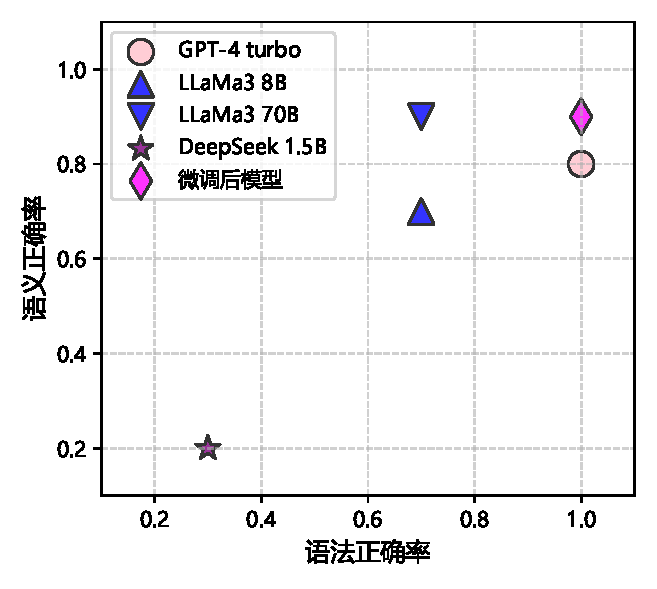
\includegraphics{figures/syntactics_and_semantics.pdf}
    \caption{各模型的语法正确率及语义正确率}
    \label{fig:syntactics_and_semantics}
\end{figure}
\begin{table}
    \centering
    \begin{tabular}{lcc}
        \toprule
        \textbf{模型} & \textbf{语法正确率} & \textbf{语义正确率} \\
        \midrule
        GPT-4 turbo & 1 & 0.8 \\
        Llama3 8B & 0.7 & 0.6 \\
        Llama3 70B & 0.7 & 0.8 \\
        DeepSeek R1 1.5B & 0.5 & 0.6 \\
        \midrule
        微调后模型 & 0.8 & 0.8 \\
        \bottomrule
    \end{tabular}
    \caption{各模型在语法和语义方面的对比分析}
    \label{fig:overall_syntactics_semantics}
\end{table}
\begin{table}[h]
    \centering
    \renewcommand{\arraystretch}{1.2}
    \setlength{\tabcolsep}{5pt}
    \resizebox{\textwidth}{!}{
    \begin{tabular}{lcccccccccccc}
        \toprule
        \multirow{2}{*}{模型} & \multicolumn{2}{c}{基础存在性} & \multicolumn{2}{c}{三维空间关系} & \multicolumn{2}{c}{多跳推理} & \multicolumn{2}{c}{多参考系} & \multicolumn{2}{c}{动态反事实} & \multicolumn{2}{c}{对抗性样本} \\
        \cmidrule(lr){2-3} \cmidrule(lr){4-5} \cmidrule(lr){6-7} \cmidrule(lr){8-9} \cmidrule(lr){10-11} \cmidrule(lr){12-13}
        & \textit{语法} & \textit{语义} & \textit{语法} & \textit{语义} & \textit{语法} & \textit{语义} & \textit{语法} & \textit{语义} & \textit{语法} & \textit{语义} & \textit{语法} & \textit{语义} \\
        \midrule
        GPT-4.0 turbo & 1 & 0.9 & 1 & 0.7 & 1 & 0.9 & 1 & 0.8 & 1 & 0.7 & 1 & 0.8 \\
        LLama3 8B & 0.9 & 0.6 & 0.7 & 0.5 & 0.8 & 0.6 & 0.6 & 0.7 & 0.5 & 0.7 & 0.7 & 0.5 \\
        LLama3 70B & 0.6 & 0.7 & 0.7 & 0.7 & 0.7 & 0.9 & 0.7 & 0.9 & 0.6 & 0.8 & 0.8 & 0.8 \\
        DeepSeek R1 1.5B & 0.5 & 0.6 & 0.7 & 0.5 & 0.6 & 0.6 & 0.4 & 0.7 & 0.4 & 0.5 & 0.5 & 0.7 \\
        \midrule
        \textbf{微调模型} & 1 & 0.9 & 0.8 & 1 & 0.6 & 0.9 & 0.9 & 0.8 & 0.9 & 0.8 & 0.6 & 0.4 \\
        \bottomrule
    \end{tabular}
    }
    \caption{不同模型在各问题类型上的语法正确率和语义正确率的对比}
    \label{tab:semantics_comparison}
\end{table}
\section{迭代反馈与规则修正}
迭代反馈模块是整个神经符号集成管道的核心部分,其主要功能在于提升由LLM生成的ASP程序的正确性和可执行性。
本文所提出的迭代反馈机制结合了自然语言解析、逻辑程序生成与符号求解三大过程,其整体流程可以描述为:
初步生成、逻辑程序执行、错误信息反馈、程序修正,直至达到预设的迭代次数或程序满足执行要求为止。
\subsection{反馈流程概述}
首先,LLM根据输入的自然语言描述生成初始的ASP程序,并将该程序交由Clingo求解器进行执行。
若在执行过程中出现任何错误(例如语法错误、变量命名不一致、或逻辑不严谨导致的求解失败),C
lingo将输出相应的错误信息。这些错误信息作为反馈被传递给LLM,指导其对初始生成的ASP程序进行针对性修正。
修正后的ASP程序再次输入Clingo求解器执行,如此循环最多进行三次,最终输出经过优化的ASP程序,
用于后续的正式推理。
\subsection{错误类型与修正策略}
不同类型的错误信息对应着ASP程序中不同的问题,因此需要采用不同的修正策略。
具体来说,本文设计了多套提示模板,用以指导LLM针对性地进行程序修正,其主要错误类型包括:
\begin{enumerate}
    \item 解析错误:如语法错误、未定义谓词、或不符合ASP语法要求的结构错误。针对该类错误,提示模板会明确指出错误的所在位置及其可能原因,并要求LLM调整相应的语法结构。
    \item 基础化错误:主要涉及变量命名不一致或不匹配等问题。此时,提示模板会强调变量的统一性和正确性,要求LLM对变量命名进行标准化处理。
    \item 求解阶段错误:包括过度约束或逻辑矛盾导致的求解失败。对于这类问题,提示模板将引导LLM重新审视程序中约束条件和规则之间的逻辑关系,并做出必要的修改。
\end{enumerate}
每一轮反馈过程中,LLM都将结合Clingo返回的错误信息和预定义的提示模板进行针对性修正,从而使生成的ASP程序在下一轮执行中更趋于正确和可执行。
\subsection{DSPy托管LLM调用}
为了高效管理这一LLM与ASP求解器之间的复杂的反馈交互过程,本文采用了DSPy框架。DSPy具备以下优势:
(1)模块化管理:DSPy将整个反馈流程拆分为若干功能模块,如ASP程序生成、错误信息解析、
提示模板更新及程序修正等。模块之间通过明确定义的接口进行通信,保证了信息的准确传递和记忆保留,
从而实现参数的自适应调整和流程优化。
(2)自动化优化:DSPy支持对LLM提示词及参数进行自动优化,极大地降低了人工调试的工作量。
在多次与LLM交互后,系统能够根据反馈动态调整提示模板,
最终得到一个较优的提示方案,以提高整体系统的修正效率和程序可执行率。
(3)日志记录与调试:为了便于调试和系统性能分析,
DSPy在整个反馈过程中对各模块的输出日志进行详细记录,包括错误信息、状态提示以及每一轮迭代的修正详情。
\subsection{DSPy优化器选择}
本文根据公开资料,对比了DSPy框架中提供的三种优化器的适用任务及场景,
如表\ref{tab:optimizer_comparison}所示。最终,本文选择了BootstrapFewShot优化器,其主要理由如下:
(1)标注成本低:传统的人工标注ASP事实需要较长时间(平均每个样本约3.5分钟),而BootstrapFewShot优化器针对少样本场景设计,仅需15-20个标注样本即可启动优化。
(2)分层次优化:BootstrapFewShot优化器将优化过程拆分为“教师优化”和“学生训练”两个阶段。教师优化阶段负责生成高质量的示例,而学生训练阶段则通过知识蒸馏完成对提示模板的优化,以确保整体修正效果的提升。
(3)资源控制:该优化器支持限制最大错误次数和迭代轮数,避免了无限循环和资源浪费,从而提高系统的稳定性与效率。

基于本文有限的标注样本和实际应用需求,选择BootstrapFewShot优化器能够在保证优化效果的同时,
大幅提高反馈迭代的效率和系统的总体性能。
\begin{table}[htbp]
\centering
\caption{Dspy 框架支持的优化器比较}
\label{tab:optimizer_comparison}
\begin{tabular}{|>{\raggedright}p{4cm}|>{\raggedright}p{8cm}|>{\raggedright\arraybackslash}p{4cm}|}
\hline
\textbf{优化器名称} & \textbf{主要功能} & \textbf{适用场景} \\
\hline
BootstrapFewShot & 通过在提示中自动生成并包含优化示例来扩展签名。 & 少样本学习 \\
\hline
BootstrapFewShot-
WithRandomSearch & 在 BootstrapFewShot 的基础上,对生成的示例进行多次随机搜索,选择优化后的最佳程序。 & 少样本学习,需要更高精度 \\
\hline
MIPRO & 在每个步骤中生成指令和少量示例,使用贝叶斯优化来有效地搜索模块中的生成指令和示例空间。 & 需要复杂指令和示例优化的场景 \\
\hline
BootstrapFinetune & 将基于提示的 DSPy 程序提炼为较小语言模型的权重更新,微调底层大型语言模型以提高效率。 & 需要微调模型以提高效率的场景 \\
\hline
\end{tabular}
\end{table}
\section{规则蒸馏}
经过迭代反馈修正后的ASP编码,已经能够顺利通过Clingo求解器执行,同时在语法和语义上保证正确。然而,回答部分可见性的问题,除了问题及其对应的图像中的
知识以外,还需要利用一些已有常识作为补充。规则蒸馏的目的在于,利用LLM的知识和已有ASP知识库的知识,对迭代反馈修正后得到的
ASP编码进行补全,减轻知识工程师手动编写规则的负担,最终得到解决问题所需的足够的ASP规则,供后续Clingo求解器
使用。

本模块的技术路径如下:模块首先对输入的
当系统检测到现有的ASP规则集无法推导出问题的正确答案时,将会。
\subsection{预提示}
预提示的作用是,为LLM提供背景信息和任务说明。具体而言,预提示包括以下内容:
\begin{enumerate}[itemsep=0pt,parsep=0pt]
\item \textbf{任务介绍}:首先简要说明VQA任务的背景,告诉LLM任务的性质——给定一个问题、一个图像和它们的描述,生成相应的答案。
\item \textbf{语言语法}:介绍ASP规则的基本语法和约定。具体而言,ASP使用了一些类似于逻辑程序设计的语法,如 :-(表示规则的条件)和 not(表示否定)。
\item \textbf{场景与问题解释}:解释如何将图像场景和问题转换成ASP的表示方式。
\item \textbf{答案格式}:告诉LLM如何表示和返回问题的答案。
\item \textbf{初始ASP理论}:提供一个初始的ASP理论,它包括一些能够回答某些问题的规则,但可能不完全覆盖所有问题。
\end{enumerate}

该机制通过增量式规则扩展实现ASP知识库的动态演进:每当系统识别出现有理论无法推导正确结果时,
会触发LLM的规则生成模块,输出符合ASP语法的逻辑规则补充到ASP知识库中。
整个过程形成“问题识别-规则生成-理论扩展”的闭环优化路径。

以下\ref{distillation-prompt}为节选的部分提示词,可作为参考。
\begin{lstlisting}[label=distillation-prompt]
你的任务是对ASP知识库进行维护,通过动态更新规则确保其能够解答各类问题。ASP知识库中的现有规则已能够满足对部分问题的处理需要,
需根据输入的问题的ASP表示进行增量式规则拓展。输入提示将包含一个或多个采用ASP表示形式的问题。请严格遵守以下规则:

1. 仅输出新增的ASP规则。
2. 禁止将事实作为规则添加。不允许在规则头(head)中使用具体常量实例。
3. 将规则的泛化程度实现最大化。你输出的规则应具备以下特征:使用大写字母变量(如X,Y,Z)替代具体常量,通过谓词逻辑建立抽象关系而非具体实例关联。
4. 完全禁用自然语言。你的输出中,不得出现任何自然语言成分,包括:错误提示信息、代码注释说和解释性文字。
\end{lstlisting}
\subsection{规则生成}
在预设提示的指导下,规则生成是知识蒸馏的核心部分。
在向LLM进行预提示之后,将迭代反馈后的ASP规则和视觉场景理解模块得到的图像描述ASP规则合并,一同作为附加输入,提示LLM。
此后LLM根据提示,推断出新的ASP规则。这些规则一方面用于后续的Clingo求解器,进行推理;另一方面,用于补充到ASP知识库中,增强神经符号框架的推理能力。

生成的规则是尽可能一般化的规则,即包含更多的变量和较少的常量,以便可以适用于更广泛的情况。
例如,如果问题是“这只杯子是什么颜色?”,LLM可能会生成以下ASP规则:
\begin{lstlisting}
color_of_cup(Color) :- object(Cup), has_attr(Cup, color, Color), class(Cup, cup).
\end{lstlisting}
这条规则表示:“如果某个物体是杯子,并且它有颜色属性,那么我们可以推理出它的颜色”。

为了对规则蒸馏LLM进行训练,补充ASP知识库,本文在对神经符号框架进行初始化时,采用了GQA数据集以构建原始ASP知识库。
对GQA数据集中的问答数据进行预处理后,每条数据均以(问题,场景,答案)的三元组形式给出,数据集中的实例被用来检测当前ASP理论的不足,
并引导LLM生成补充规则,以便在语法和语义检查通过后将新规则融入系统中,从而提升整体推理能力。 
\subsection{规则验证}
在LLM生成新规则后,接下来的步骤是验证这些规则是否正确。这一过程包括语法检查和语义检查。

生成的规则必须符合ASP的语法要求。如果规则存在语法错误,例如拼写错误或格式不对,ASP解析器将无法解析这些规则。
在这种情况下,系统会将错误信息反馈给LLM,并要求LLM进行修正。

语法检查通过后,下一步是检查规则是否能够正确推理出答案。这意味着通过执行这些规则,ASP推理引擎是否能够得到与问题期望答案相符的推理结果。
例如,假设输入问题是“图中的杯子是什么颜色?”,而答案是“红色”。如果LLM生成的规则无法推导出这个结果,系统会向LLM反馈推理结果与预期答案不符,并要求其修正规则。

在语义检查失败时,系统会将实际推理结果和期望答案作为反馈,向LLM提出修改建议。LLM根据反馈修正其生成的规则,直到推理结果正确为止。
\subsection{回归测试}
回归测试的目的是在扩展ASP理论的同时,确保新规则不会导致旧问题的答案错误。这一设计主要基于以下几方面的考量:
\begin{enumerate}[itemsep=0pt,parsep=0pt]
\item \textbf{维护系统稳定性和一致性}:​在软件工程中,回归测试被广泛应用于验证新代码的引入是否影响现有功能的正确性。
类似地,在VQA系统中,每当通过知识蒸馏添加新规则时,需要确保这些规则不会干扰系统对先前问题的解答。
\item \textbf{应对模型更新带来的潜在风险}:​知识蒸馏的过程涉及从教师模型向学生模型传递知识,可能导致学生模型的行为发生变化。
通过回归测试,可以检测并防止新知识引入后对模型性能的负面影响。
\item \textbf{借鉴软件开发中的最佳实践}:​在软件开发中,回归测试是确保新功能或修改不会引入新错误的关键步骤。
将这一理念应用于VQA系统,有助于在不断扩展和优化系统的同时,保持其可靠性和准确性。
\end{enumerate}

回归测试的具体步骤如下:基于更新后的ASP理论,重新执行所有历史测试用例,确保所有旧问题仍然能得到正确答案。
如果某个旧问题的答案被破坏,则回退到先前的ASP理论,并要求LLM重新修正生成的规则。

通过上述设计,回归测试在VQA系统的知识蒸馏过程中起到了关键的质量保证作用,确保系统在不断学习和扩展的同时,保持其稳定性和可靠性。
\subsection{示例选择策略}
VQA数据集中包含数百万个样例,如果直接处理所有样例,既耗时又可能引入冗余信息。
因此,为了提高蒸馏效率,本文提出了样例选择策略,以减少无关数据的干扰。具体而言,包括以下两种方法:
\begin{enumerate}[itemsep=0pt,parsep=0pt]
\item \textbf{谓词计数策略}:该策略根据ASP问题表示中谓词的数量对实例进行分组。​分组方法是:​统计每个问题表示中出现的谓词数量,并将具有相同谓词数量的问题归为一组。​​通过这种分组方式,可以根据问题的复杂度(即涉及的谓词数量)来选择示例。
​这有助于LLM在训练过程中逐步学习,从处理简单问题(谓词数量少)开始,逐步过渡到复杂问题(谓词数量多),从而提高生成规则的准确性和泛化能力。
\item \textbf{谓词相关性策略}:该策略根据ASP问题表示中涉及的具体谓词对实例进行分组。分组方法是:​识别每个问题表示中出现的谓词,并将包含相同谓词的问题归为一组。​
通过这种分组方式,可以确保LLM针对特定谓词学习相关规则。​这有助于LLM深入理解每个谓词的作用和使用场景,从而生成更精确的ASP规则,提升VQA系统在处理涉及特定谓词的问题时的表现。
\end{enumerate}

谓词计数策略的设计借鉴了课程学习(Curriculum Learning)的思想。
​课程学习是一种训练策略,强调按照从易到难的顺序逐步引入训练样本,以提高模型的学习效果。
谓词计数策略通过问题复杂度的分层,体现了课程学习的理念,使模型能够在逐步增加的复杂度中稳定学习。

​在自然语言处理和知识表示领域,基于谓词的特征选择方法被广泛应用于文本分类和信息检索等任务。
谓词相关性策略吸取了这一方法的经验,通过关注问题中涉及的具体谓词,利用领域知识进行特征选择,确保模型关注于最相关的信息,提高推理的准确性。
\subsection{批量优化}
为了进一步提高效率,论文还提出了批量优化策略,即一次性给LLM多个示例,而不是逐个示例地生成规则。
这一策略借鉴自Ge\cite{ge2021selfdistillationbatchknowledgeensembling}等人提出的批量知识集成的自蒸馏方法。
​在知识蒸馏领域,批量知识集成方法通过在同一小批量内传播和整合样本间的知识,生成更精确的软目标,从而提升模型性能。
此外,自蒸馏方法利用模型自身的预测作为训练目标,减少对外部教师模型的依赖,简化训练流程。

采用批量优化策略,具有以下几点突出优势:
\begin{enumerate}[itemsep=0pt,parsep=0pt]
\item \textbf{提高训练效率}:​通过在同一批次内处理多个样本,模型可以并行学习不同样本的特征和模式,减少训练时间。
\item \textbf{增强模型泛化能力}:批量优化允许模型在一个批次内接触多样化的数据,帮助模型学习更广泛的特征表示,从而提升对未见数据的适应能力。
\item \textbf{优化资源利用}:通过批量处理,能够更有效地利用计算资源,减少训练过程中的开销。
\end{enumerate}

综合来看,批量优化策略通过借鉴批量知识集成和自蒸馏等方法,旨在提升知识蒸馏过程中的训练效率和模型性能。
\section{ASP推理}
ASP推理阶段中,ASP求解器接收经过优化后的ASP查询语句、视觉场景理解模块提取的ASP事实以及已有常识的ASP表示,进行逻辑推理,最终获得答案。
本文使用Clingo求解器来进行求解,其工作过程分为基础化(grounding)阶段和求解(solving)阶段。

基础化阶段将ASP程序中的变量替换为常量,生成一个新的ASP程序。Clingo
通过使用内置的基础化器分析程序,生成所有可能的规则。例如,对规则
$a(X) :- b(X), not c(X).$,其将被展开为所有可能的值为X的实例。

求解阶段中,Clingo采用类似SAT求解器的冲突驱动答案集求解(CDNL)方法。CDNL方法通过迭代地添加约束,直到找到一个满足所有约束的解,或者证明无解。
具体而言,Clingo基于如下步骤进行求解:(1)初始化。从空分配开始(没有原子被标记为真);
(2)选择与分配。选择一个未分配的原子,猜测其真值为真或假;
(3)传播。根据当前分配和规则,推导其他原子的真值。例如,若规则$a :- b, not c.$满足,b为真且c不在答案集中,则a必须为真;
(4)冲突检测。若分配导致规则冲突(如与已有的约束条件相抵触),记录冲突原因;
(5)回溯与学习。若发生冲突,回溯到之前的选择点,学习冲突子句以避免未来类似错误;
(6)验证。当所有原子分配完成后,检查是否为答案集,即确保它是程序的模型,且最小化(无子集也能满足规则)。

相比其它的ASP求解器,Clingo在以下几个方面进行了优化:(1)从冲突中学习
新的规则,为将来进一步的搜索提供指导;(2)使用多线程实现并行化,同时搜索
多个路径,加速求解过程;(3)使用启发式方法决定分配顺序,例如优先选择高影响力的原子;
(4)预测可能发生的冲突,选择可能导致冲突的原子优先分配,减少搜索空间。
\section{求解结果翻译}
经过Clingo得到的输出结果,以ASP谓词表示,对用户而言并不友好。需要将其转为自然语言。
Clingo输出的是由逻辑谓词构成的答案集,例如谓词\textbf{is(A, left, B)}表示“A位于B的左侧”。
由于正常情况下,Clingo输出的都是预定义的谓词,故采用构造同义词字典的方案,将ASP中的逻辑谓词与自然语言
表述对应起来。LLM可基于这些模板对解析后的逻辑结果进行填充和修正,生成标准化且易于理解的描述。
\section{实验与结果分析}
\subsection{对比试验}
为全面评估神经符号框架的有效性以及泛化能力,本文选取了目前主流的三种LLM:DeepSeek R1、
Llama3和GPT-4 turbo,在其上应用神经符号框架,进行对比。以上既包含DeepSeek这类轻量级专用模型,
也涵盖GPT-4 turbo这类通用型先进系统,而Llama3性能和效率之间取得了平衡,属于居中水平的模型。通过
在多个基座上进行实验,证明神经符号框架对不同LLM的泛化能力。

基线模型一选取直接提示VLM的方式,即直接将自然语言问题和图像输入到VLM中,并不给予任何的额外提示。
直接提示VLM的方式虽然简单,却是评估模型的关键基准,因为直接提示方法能够反映模型在没有任何
外部推理辅助机制的情况下,自身对空间问题的处理能力。

基线模型二采用“事实+规则”的提示方法。该方法的核心思路是:指示LLM使用预先定义的谓词,将输入的自然语言问题转换为结构化事实,然后LLM应用相关逻辑
规则,通过自然语言推理答案。
“事实+规则”的提示方法满足了将原始自然语言问题转为结构化符号表示,以配合视觉场景理解所得的ASP事实以及原有常识,共同进行推理的核心需求。同时,
该方法使用具有精确参数结构的谓词对LLM进行提示,使得LLM可以创建一致的中间态的知识表示,为问题解答提供便利。综合来看,“事实+规则”的提示方法作为一种
简化流程,既保留了形式化推理的优势,同时能够避免在生成ASP程序时和LLM进行多次交互,进而降低对计算资源的要求,降低了成本,也减少了对外部求解器的依赖。

实验结果见表\ref{tab:overall_comparison},本文提出的神经符号框架在DeepSeek R1、LLama3和GPT-4.0 turbo上均超过了两种比较基准方法,证明大语言模型与逻辑推理结合对于解决
复杂空间推理问题的有效性。

\begin{table}[h]
    \centering
    \small  % 调整字体大小(可选:\footnotesize 更紧凑)
    \renewcommand{\arraystretch}{1.2}  % 增加行距
    \setlength{\tabcolsep}{5pt}  % 调整列间距
    \resizebox{\textwidth}{!}{  % 让表格自适应页面宽度
    \begin{tabular}{lcccccc}
        \toprule
        \textbf{模型及方法} & \textbf{基础存在性问题} & \textbf{三维空间关系问题} & \textbf{多跳推理问题} & \textbf{多参考系问题} & \textbf{对抗性样本问题} & \textbf{总体} \\
        \midrule
        \multicolumn{7}{c}{\textbf{DeepSeek R1}} \\  
        直接提问 & 60.5 & 38.2 & 74.5 & 78.2 & 48.2 & 59.9 \\
        事实+规则提示方法 & 69.7 & 47.3 & 80.6 & 80.9 & 56.6 & 67.0 \\
        神经符号框架方法 & 77.8 & 58.9 & 85.4 & 81.8 & 42.8 & 69.3 \\
        \midrule
        \multicolumn{7}{c}{\textbf{Llama3}} \\  
        直接提问 & 68.4 & 26.9 & 65.7 & 72.5 & 55.8 & 57.9 \\
        事实+规则提示方法 & 75.3 & 46.8 & 70.2 & 81.4 & 57.1 & 66.2 \\
        神经符号框架方法 & 79.1 & 53.1 & 83.3 & 80.5 & 60.8 & 71.4 \\
        \midrule
        \multicolumn{7}{c}{\textbf{GPT-4.0 turbo}} \\  
        直接提问 & 77.2 & 45.4 & 60.9 & 57.6 & 58.2 & 59.9 \\
        事实+规则提示方法 & 85.3 & 54.3 & 68.2 &61.5 & 50.4 & 64.0 \\
        神经符号框架方法 & 91.1 & 65.6 & 80.5 & 72.7 & 64.8 & 74.9 \\
        \bottomrule
    \end{tabular}
    }
    \caption{不同模型及方法在各问题类型上的表现}
    \label{tab:overall_comparison}
\end{table}

\subsection{消融实验}
尽管LLM在语义解析任务中表现出色,但其生成的ASP程序的正确率仍有较大的提升空间。Feng\cite{feng2024language}等人的研究表明,将自然语言直接转为逻辑规则的
成功率一般较低。而神经符号框架通过在LLM和外部ASP求解器之间设立反馈循环机制,使LLM能够根据ASP求解器在试图求解ASP程序之前的语法检查结果,对生成的ASP程序
中的错误进行修正,极大提高了将自然语言问题转为ASP程序的准确率。

为进一步探讨神经符号框架的迭代反馈机制的作用,本文重点关注ASP求解器执行过程中常发生的三类主要错误:解析错误、实例化失败以及求解阶段失败。
另外,即便生成的ASP程序执行成功,也有很大可能由于自然语言问题与LLM生成的ASP程序之间不一致,而产生与真实答案偏离的结果。

在测试中,迭代反馈机制显著提升了所有模型的性能。如图\ref{fig:ablation}所示,经过两轮迭代反馈之后,DeepSeek R1的可执行率从51.3\%提升到了84.2\%,LLama3的可执行率从60.2\%提升到了89.7\%
,GPT-4.0 turbo的可执行率从64.6\%提升到了91.1\%。
在准确率方面,DeepSeek R1的准确率从57.8\%提升到了79.3\%,LLama3的准确率从61.1\%提升到了85.7\%,GPT-4.0 turbo的准确率从69.7\%提升到了93.4\%。
以上结果表明,LLM与ASP求解器之间的迭代反馈机制能有效解决自然语言到逻辑程序的转换过程中面临的问题。对准确率和可执行率的提升,主要集中在
第一轮迭代反馈中,此后继续迭代的效果呈现边际递减趋势。由于计算资源有限,本次消融实验仅进行了三轮。实验结果有力证明,迭代反馈机制在提升ASP程序的可执行率和
正确率方面具有明显效果,充分验证了神经符号方法的有效性。

\begin{figure}
    \centering
    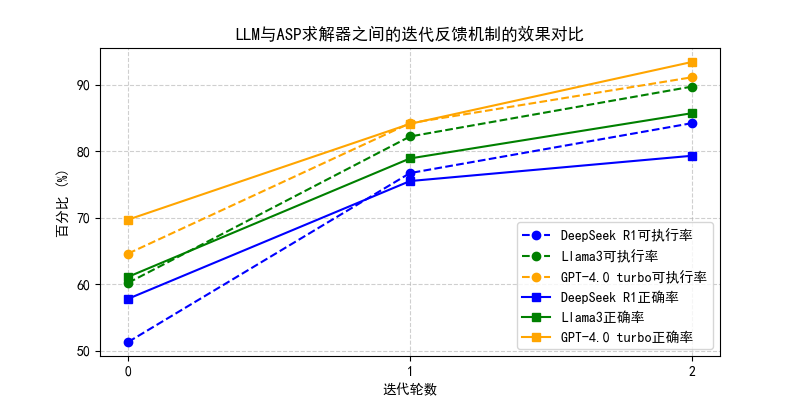
\includegraphics[width=\textwidth]{ablation.png}
    \caption{LLM与ASP求解器之间的迭代反馈机制的效果对比}
    \label{fig:ablation}
\end{figure}

\section{本章小结}
本章详细介绍了神经符号框架的整体架构设计与实现过程,阐述了从视觉场景理解、语义解析、迭代反馈与规则修正
到规则蒸馏,
再到最终的ASP推理的完整流水线。首先,框架总体架构明确了LLM在语义解析和反馈优化中的双重作用,
为复杂空间关系推理提供了有效支撑。接着,在视觉场景理解部分,本文基于GLIP模型实现了目标检测,
并通过中心点与深度信息提取物体的二维及三维位置信息,再结合空间关系提取技术构建场景图,
并将提取的信息转化为ASP事实,为后续逻辑推理打下坚实基础。

在语义解析模块中,利用LLM的上下文学习能力,通过微调生成与自然语言问题对应的ASP程序,
设计了多种ASP模板以覆盖基础存在性、三维空间关系、多跳推理、多参考系、动态反事实以及对抗性样本等问题类型。
实验结果表明,经过微调和DSPy框架支持下的提示优化,生成的ASP查询在语法与语义上均取得了较高准确率,
验证了LLM在语义解析任务中的有效性。

随后,通过迭代反馈与规则修正模块,系统实现了LLM与ASP求解器之间的闭环交互:
Clingo求解器对生成的ASP程序进行执行检查,并反馈错误信息,LLM据此优化ASP程序,
经过多轮迭代后显著提升了程序的可执行率和语义正确率。接着,通过规则蒸馏模块,以迭代反馈与规则修正模块得到
的ASP代码和视觉场景理解得到的ASP代码为输入,以ASP知识库为基础,调用LLM对ASP规则进行补充,同时对ASP知识库进行
更新完善。
最后,在对比试验和消融实验中,
本文综合比较了不同LLM模型和提示方法的表现,验证了神经符号框架在处理复杂空间推理问题上的泛化能力与优势,
同时也证明了迭代反馈机制对整体性能提升的重要作用。

总体来说,本章不仅构建了一个完整而高效的神经符号推理流水线,而且通过详细实验与消融分析,
验证了各模块间协同工作的有效性,为后续基于逻辑推理的VQA系统提供了坚实的理论和实践基础。